\section{Background: CvRDTs and eventual consistency}\label{s:distributed-cvrdts}

Shapiro \etal~\cite{crdts, crdts-tr} define an \emph{eventually
  consistent} object as one that meets three conditions.  One of these
conditions is the property of \emph{convergence}: all correct replicas
of an object at which the same updates have been delivered eventually
have equivalent state.  The other two conditions are \emph{eventual
  delivery}, meaning that all replicas receive all update messages,
and \emph{termination}, meaning that all method executions terminate
(we discuss methods in more detail below).

Shapiro \etal~further define a \emph{strongly eventually consistent}
(SEC) object as one that is eventually consistent and, in addition to
being merely convergent, is \emph{strongly convergent}, meaning that
correct replicas at which the same updates have been delivered have
equivalent state.\footnote{ Strong eventual consistency is not to be
  confused with strong consistency: it is the combination of eventual
  consistency and strong convergence.  Contrast with ordinary
  convergence, in which replicas only \emph{eventually} have
  equivalent state.  In a strongly convergent object, knowing that the
  same updates have been delivered to all correct replicas is
  sufficient to ensure that those replicas have equivalent state,
  whereas in an object that is merely convergent, there might be some
  further delay before all replicas agree.}  A \emph{conflict-free
  replicated data type} (CRDT), then, is a data type (\ie, a
specification for an object) satisfying certain conditions that are
sufficient to guarantee that the object is SEC.  (The term ``CRDT'' is
used interchangeably to mean a specification for an object, or an
object meeting that specification.)

\ifdefined\DISSERTATION
\begin{wrapfigure}{l}{1.4in}
\vspace{-2em}
\begin{center}
  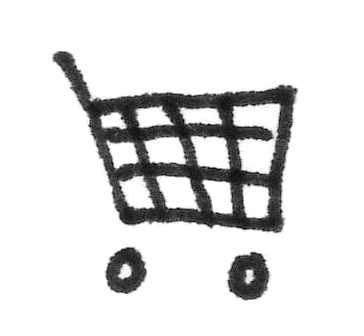
\includegraphics[scale=0.2]{../illustrations/shopping-cart}
\end{center}
\vspace{-1.5em}
\end{wrapfigure}
\fi 

There are two ``styles'' of specifying a CRDT: \emph{state-based},
also known as \emph{convergent}\footnote{There is a potentially
  misleading terminology overlap here: the definitions of convergence
  and strong convergence above pertain not only to CvRDTs (where the C
  stands for ``Convergent''), but to \emph{all} CRDTs.}; or
\emph{operation-based} (or ``op-based''), also known as
\emph{commutative}.  CRDTs specified in the state-based style are
called \emph{convergent replicated data types}, abbreviated
\emph{CvRDTs}, while those specified in the op-based style are called
\emph{commutative replicated data types}, abbreviated \emph{CmRDTs}.
Of the two styles, we focus on the CvRDT style in this paper because
CvRDTs are lattice-based data structures and therefore amenable to
threshold queries---although, as Shapiro \etal~show, CmRDTs can
emulate CvRDTs and vice versa.

\subsection{State-based objects}

In the Shapiro \etal~model, a \emph{state-based object} is a tuple
$(S, s^0, q, u, m)$, where $S$ is a set of states, $s^0$ is the
initial state, $q$ is the \emph{query method}, $u$ is the \emph{update
  method}, and $m$ is the \emph{merge method}.  Objects are replicated
across some finite number of processes, with one replica at each
process, and each replica begins in the initial state $s^0$.  The
state of a local replica may be queried via the method $q$ and updated
via the method $u$.  Methods execute locally, at a single replica, but
the merge method $m$ can merge the state from a remote replica with
the local replica.  The model assumes that each replica sends its
state to the other replicas infinitely often, and that eventually
every update reaches every replica, whether directly or indirectly.

The assumption that replicas send their state to one another
``infinitely often'' refers not to the \emph{frequency} of these state
transmissions; rather; it says that, regardless of what event (such as
an update, via the $u$ method) occurs at a replica, a state
transmission is guaranteed to occur after that event.  We can
therefore conclude that all updates eventually reach all replicas in a
state-based object, meeting the ``eventual delivery'' condition
discussed above.  However, we still have no guarantee of strong
convergence or even convergence.  This is where Shapiro \etal's notion
of a CvRDT comes in: a state-based object that meets the criteria for
a CvRDT is guaranteed to have the strong-convergence property.

A \emph{state-based} or \emph{convergent} replicated data type (CvRDT)
is a state-based object equipped with a partial order $\leq$, written
as a tuple
$(S, \leq, s^0, q, u, m)$, that has the following properties:
\begin{itemize}
\item $S$ forms a join-semilattice ordered by $\leq$.
\item The merge method $m$ computes the join of two
  states with respect to $\leq$.
\item State is \emph{inflationary} across updates: if $u$ updates a
  state $s$ to $s'$, then $s \leq s'$.
\end{itemize}
Shapiro \etal~show that a state-based object that meets the criteria
for a CvRDT is strongly convergent.  Therefore, given the eventual
delivery guarantee that all state-based objects have, and given an
additional assumption that all method executions terminate, a
state-based object that meets the criteria for a CvRDT is
SEC~\cite{crdts}.

\subsection{Discussion: the need for inflationary updates}

Although CvRDT updates are required to be inflationary, it is not the
case that every update must be inflationary for convergence, given our
assumption of eventual delivery.  Consider, for example, a scenario in
which replicas 1 and 2 both have the state $\{a, b\}$. Replica 1
updates its state to $\{a\}$, a non-inflationary update, and then
sends its updated state to replica 2.  Replica 2 merges the received
state $\{a\}$ with $\{a, b\}$, and its state remains $\{a, b\}$. Then
replica 2 sends its state back to replica 1; replica 1 merges $\{a,
b\}$ with $\{a\}$, and its state becomes $\{a, b\}$.  The
non-inflationary update has been lost, and was, perhaps,
nonsensical---but the replicas are nevertheless convergent.

However, once we introduce threshold queries of CvRDTs, as we will do
in the following section, inflationary updates become \emph{necessary}
for the determinism of threshold queries.  This is because a
non-inflationary update could cause a threshold query that had been
unblocked to block again, and so arbitrary interleaving of
non-inflationary writes and threshold queries would lead to
nondeterministic behavior.  Therefore the requirement that updates be
inflationary will not only be sensible, but actually crucial.

